\section{Angolo di Brewster}
\begin{figure}[h!]
    \centering
    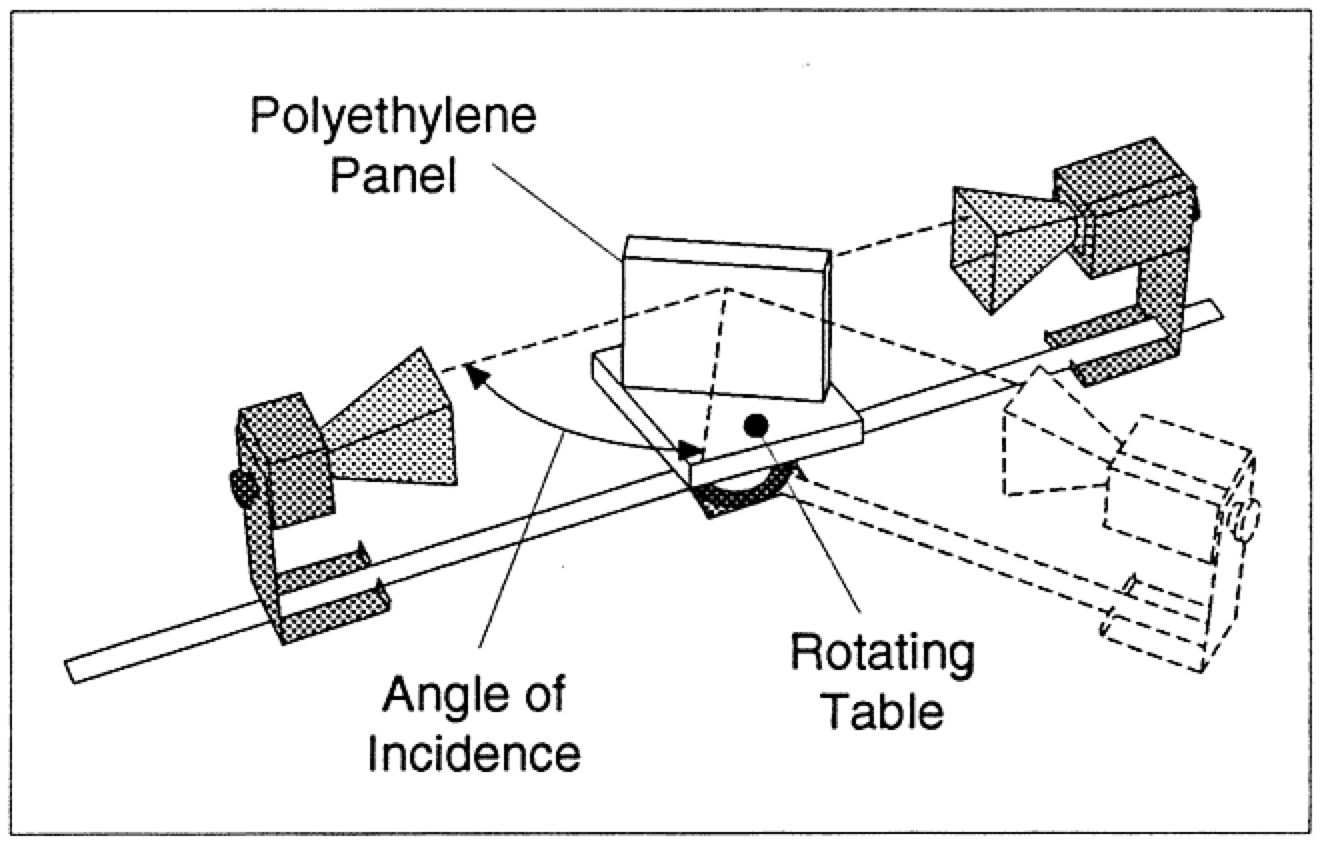
\includegraphics[scale=.3]{Immagini/Schermata 2022-04-07 alle 2.36.29 PM.png}
    \caption{Configurazione dell'apparato sperimentale per la misura dell'angolo di Brewster}
    \label{apparato browser}
\end{figure}

Obiettivo della sezione è stato quello di verificare l'angolo di Brewster.
\noindent
Abbiamo campionato per diversi angoli il valore dell'intensità, con maggiore concentrazione di campionamenti vicino al massimo.
\begin{figure}[h!]
    \centering
    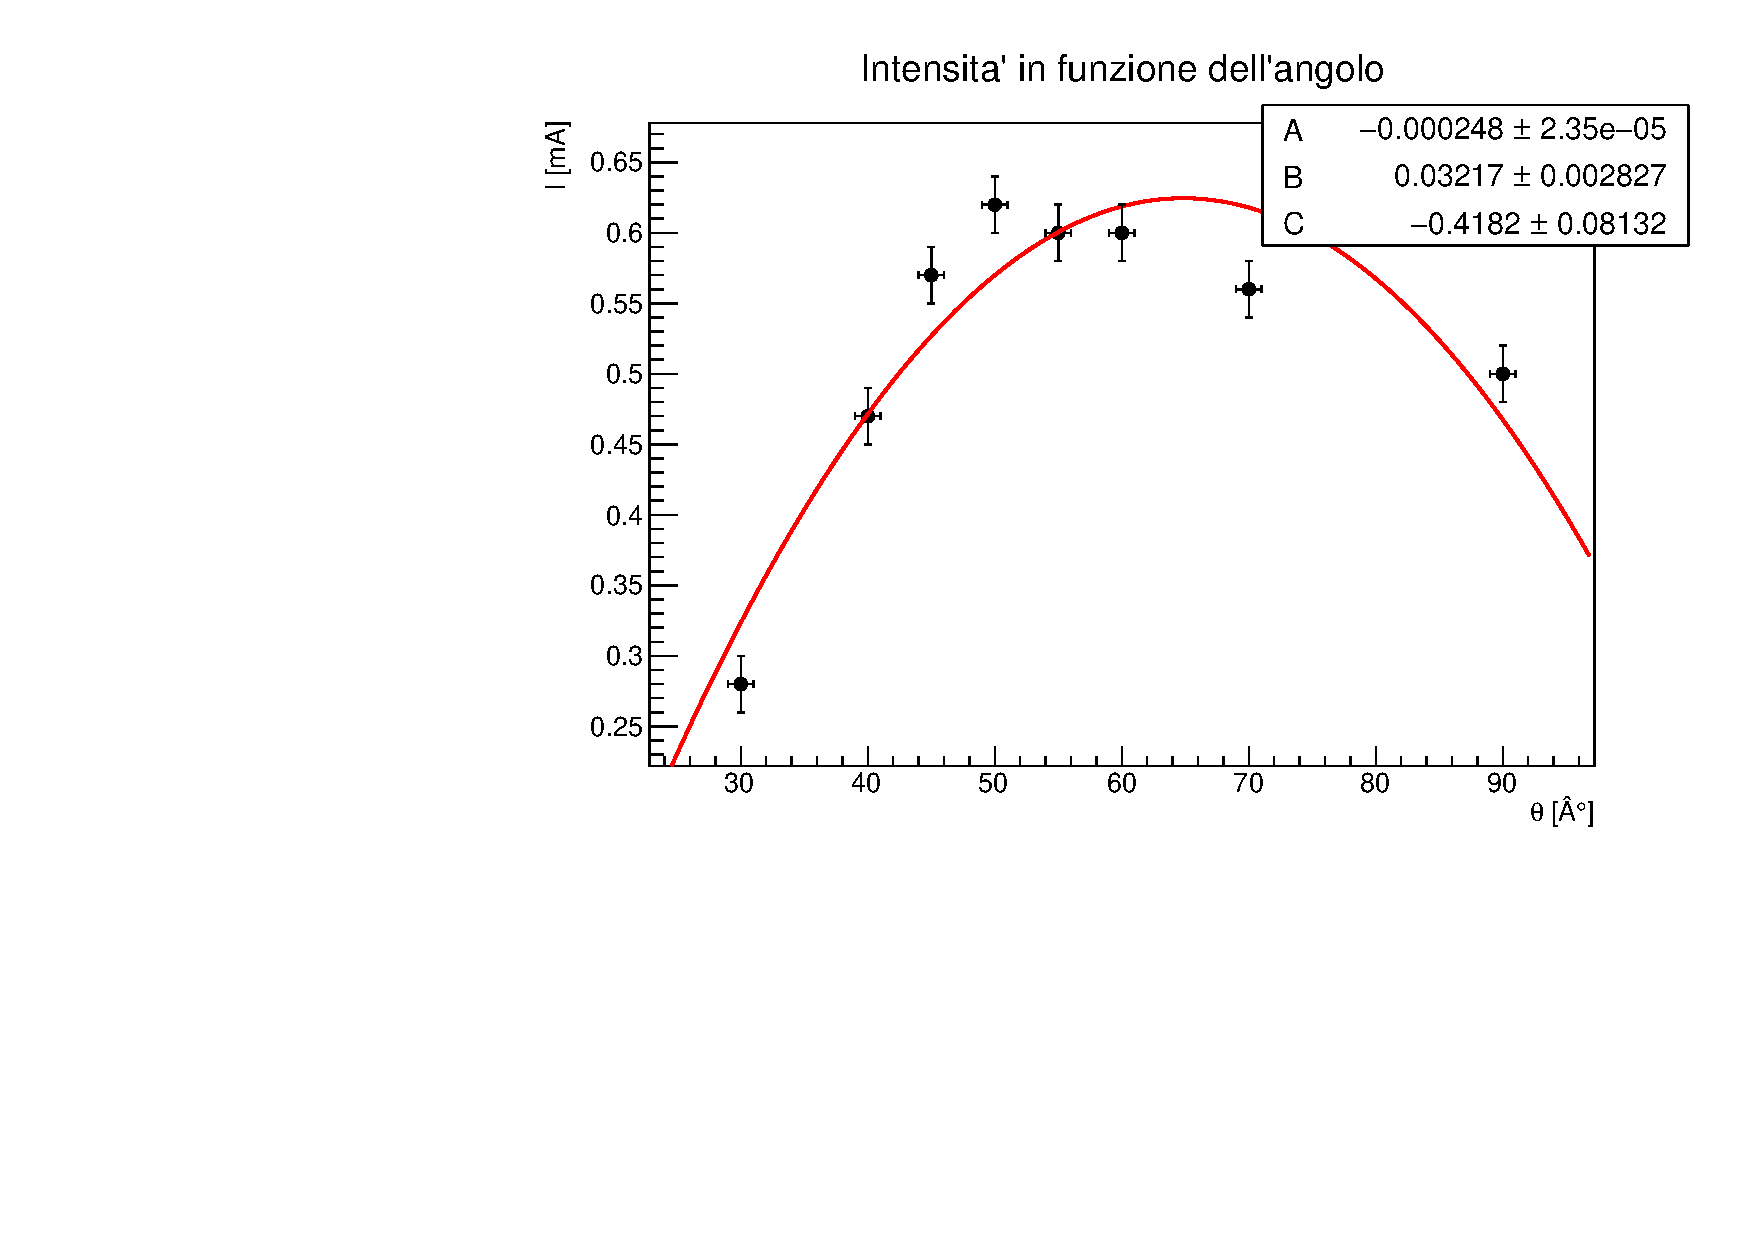
\includegraphics[scale=.5]{Immagini/browser.pdf}
    \caption{}
    \label{}
\end{figure}
Dopo aver interpolato i dati vicino a quest'ultimo, come se questi seguissero una relazione quadratica, abbiamo ricavato il massimo attraverso il calcolo analitico della derivata. Il valore ricavato è $\ang{64}\, 86'$.
Per valutare l'errore abbiamo tenuto conto della correlazione tra $A$ e $B$, calcolando la covarianza tra i due parametri. Covarianza ricavata dalla matrice di covarianza (Eq. \ref{eq 3}) dei tre parametri utilizzati per l'interpolazione.
\begin{equation}
\sigma_{ABC}=
\begin{pmatrix}
5.5232\cdot 10^{-10} & -6.5443\cdot 10^{8} &
1.7909\cdot 10^{-6}\\
\\
-6.5443\cdot 10^{-8} &
7.9896\cdot 10^{-6} & -2.2544\cdot 10^{-4}\\
\\
1.7909\cdot 10^{-6} & -2.2544\cdot 10^{-4} &
6.6125\cdot 10^{-3}\\
\end{pmatrix}
\label{eq 3}
\end{equation}

%La covarianza risulta essere di METTERE VALORE COVARIANZA, l'errore invece di METTERE VALORE ERRORE.
%fare propagazione errore sull'angolo calcolato a mano
